\section{Windowing}
The Hann (with $\alpha = 0.5$) and Hamming windows are first evaluated for the prominence of their main lobe and sidelobes
in the frequency domain on the synthetic datasets. Figure \ref{fig:clean filters} illustrates the 
performance of each of the filters on a clear sine wave with no noise. Figure \ref{fig:noisy filters}
illustrates the performance of each of the filters on the noisy simulated data with an SNR of 1.  

\begin{figure}
    \incfig[0.7]{filter_clear_comparison}
    \caption[Window filter comparison on a noise-free signal.]{Results of an \gls{fft} performed on a single frequency signal without noise without a filter,
    with a Hann window, and a Hamming window. Each of the tests correctly produces a peak near
    bin 334, the target range. The no filter option's peak is wider than the filtered options.
    The Hann window performs the best globally, with a 100 dB reduction in power when more than 40
    bin away from the target bin. The Hamming window performs significantly worse globally, with
    only a 70 dB reduction when more than 40 bins away, but has a steeper drop-off near the
    target bin, which may result in better resolution of closely spaced targets.}
    \label{fig:clean filters}
\end{figure}

\begin{figure}
    \incfig[0.7]{filter_noisy_comparison}
    \caption[Window filter comparison at SNR of 1.]{Results of an \gls{fft} performed on a single frequency signal with an SNR of 1 with no
    window filter, with a Hann window filter, and a Hamming window filter. The no filter option's
    spectral leakage acts to deform the peak at bin 334. The Hann and Hamming windows perform similarly
    globally but the Hamming window features a slightly higher peak, and less spectral leakage into
    the adjacent bins.}
    \label{fig:noisy filters}
\end{figure}

In terms of computational performance, the latency contribution of the filters does not significantly 
differ across implementations. Figure \ref{fig:latency} shows the time taken to process
a single frame of 10 000 chirps each with 767 samples, averaged over 50 runs. 

\begin{figure}
    \incfig[0.7]{filter_latency_comparison}
    \caption[Windowing stage latency across implementations.]{Latency contribution of the windowing stage to the overall pipeline. The latency does not
    significantly differ across implementations, with all implementations taking around 9-12 ms to
    process 7 670 000 samples. The insignificant difference in latency between no filter
    and filters suggests that the delay is primarily due to the overhead of handling the data.}
    \label{fig:latency}
\end{figure}

The experiments were then extended to the Blackman, Kaiser, and Taylor windows. Using dataset DS2,
the multi-receiver signal of a target sweep azimuth, elevation and range, fifteen filter 
configurations were applied to the data: \verb|Hann|, \verb|Hamming|, \verb|Blackman|, 
\verb|Kaiser6|, \verb|Kaiser8|, \verb|Kaiser10|, \verb|Kaiser12|, \verb|Taylor1_30|, 
\verb|Taylor2_30|, \verb|Taylor_3_30|, \verb|Taylor_4_30|, \verb|Taylor1_50|, \verb|Taylor2_50|
\verb|Taylor_3_50|, \verb|Taylor_4_50|. The parameter suffix of the Kaiser windows indicate the 
\(\beta\) parameter and the two suffixes of the Taylor windows indicate \(\bar{n}\) and the 
sidelobe level in -dB respectively.  

Six noise intensities were applied to the data: no noise, and SNRs of -20, -10, 
0, 10 and 20 dB. Detections at ranges where the target is not were labelled as clutter, they 
were tallied and their total power was recorded. Figures \ref{fig:recall_vs_clutter} and 
\ref{fig:recall_vs_clutter_power} illustrate the relationship between noise, windows, and their
effect on recall and clutter.  

\begin{figure}
    \incfig[0.8]{windowing_recall_vs_clutter}
    \caption[Recall vs clutter for different window functions.]{Recall vs clutter for different 
    window functions. The recall of the target detections decreases from 1 to 0.45 with increasing 
    noise, and the number of clutter detections increases with increasing noise from 3 to 12 per 
    actual truth. Window choice trades less clutter for sensitivity. The Taylor windows calibrated
    to -50dB noise achieve high recall without introducing more clutter than the other windows. The choice of window does 
    not significantly affect recall or clutter, though the Hamming window performs slightly 
    better at high SNRs.}
    \label{fig:recall_vs_clutter}
\end{figure}

\begin{figure}
    \incfig[0.8]{windowing_recall_vs_clutter_power}
    \caption[Recall vs clutter power for different window functions.]{Recall vs clutter power 
    for different window functions. While producing slightly higher clutter power, the four 
    -50 dB Taylor windows achieve higher recall than the other windows in the three noisiest 
    conditions.}
    \label{fig:recall_vs_clutter_power}
\end{figure}

\FloatBarrier
\section{Integration}
The integration stage is validated on synthetic test data from software scripts and the 
test-source mode of the AWR2243 radar chips. The results from the former illustrate the expected increase
in SNR with increasing integration window size as demonstrated in Figure \ref{fig:integration-waterfall}. 
The results from the latter illustrate no increase in SNR because the test-source mode does not generate 
any noise. Meaningfully, the results from the AWR test-source mode indicate that the integration stage 
behaves correctly on data from the radar chips, (see Figure \ref{fig:integration-waterfall-orac}). The 
subsystem can process the data at a rate of 9.8 times the incoming data rate on the desktop setup, and 
3.8 times the incoming data rate on the Xavier setup. We also find that the latency of the integration 
stage increases with the integration's factor of reduction, since in our implementation,
each thread performs all the sum operations for its corresponding range bin
(which increases with the reduction factor of the integration stage). 


\begin{figure}
    \incfig[0.57]{integration_waterfall}
    \caption[Integration on synthetic data showing SNR improvement.]{Results of the integration stage on synthetic data.
    The top window shows a low SNR waterfall plot of data, with the y-axis
    representing range samples and
    the x-axis representing chirps that are streaming into the integration stage. The
    colour indicates the power of the range bin, with yellow being the most intense.
    The output of the integration stage below has less noise, and the target
    signal is more prominent.} 
    \label{fig:integration-waterfall}
\end{figure}

\begin{figure}
    \incfig[0.57]{integration_waterfall_orac}
    \caption[Integration on AWR2243 test-source data.]{Results of the integration stage on AWR2243 test-source data.
    The 8 windows correspond to 8 channels. 128 chirps are being compressed into a single
    chirp with no noise. There is
    no change in amplitude, validating that the integration stage behaves
    correctly on radar chip data.}
    \label{fig:integration-waterfall-orac}
\end{figure}

The latency of the integration stage increases with the reduction factor of the integration stage,
as demonstrated in Figure \ref{fig:ablation-cumulative-latency}. Many of this latency is due to 
the overhead associated with handling the data and the launching the application. By finding the 
time taken
to process as a function of the number of input frames we can approximate the startup time of the 
pipeline and subtract it from the total time to find the time taken to process each frame. 
This is done with coherent integration, non-coherent integration, and no integration as a 
baseline. 
Additionally, for this trial, the pipeline has been patched to not input or output any data, just processing
empty buffers, which allows us to avoid measuring the overhead of handling the data.  

\begin{figure}
    \incfig[0.7]{integration_throughput}
    \caption[Integration stage latency per frame.]{Processing time as a function of the number 
    of input frames. The startup time of the pipeline is approximated 
    by finding the y-intercept of the line of best fit, which is 195 ms for all three scenarios. 
    The figure also illustrates that there is only a small difference between the processing time
    of either integration strategy and no integration at all, with the non-coherent integration
    taking 0.02 milliseconds more per frame than no integration, and the coherent integration. 
    }
    \label{fig:integration-latency-per-frame}
\end{figure}

Dataset DS2 sweeps az el and range in the six noise regimes, -20, -10, 0, 10 and 20dB SNR and no noise. 
SNRs were tuned to detections at the further ranges. Closer detections have higher SNRs than 
what is listed. 
Figure \ref{fig:integration-setup} illustrates the ground truths and 64 detections per ground truth
for one of the noisy scenarios. 

\begin{figure}
    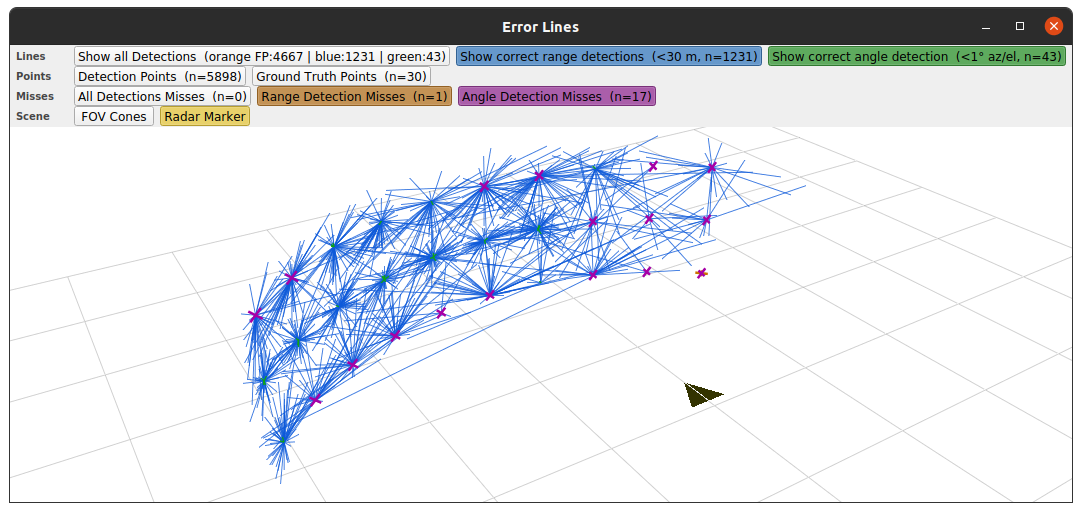
\includegraphics[width=0.9\textwidth]{integration_setup.png}
    \caption[Integration experiment ground truths and detections.]{The setup of the integration 
    stage experiment for accuracy evaluation. The figure shows the detections of a target 
    sweeping azimuth, elevation and range in a noisy scenario. Each line segment indicates the 
    ground truth on one end and the detection on the other. Purple crosses indicate ground 
    truths with no detections within 1 degree in azimuth and elevation of them. The triangle 
    marks the radar position and heading.}
    \label{fig:integration-setup}
\end{figure}

The results of the experiment are illustrated in Figures 
\ref{fig:integration-angle-recall-per-segment} and
\ref{fig:integration-RMS-position-error}.

\begin{figure}
    \incfig[0.9]{integration_angle_recall_per_segment}
    \caption[Recall Integration Experiment.]{Recall, the proportion of ground truths 
    with at least one detection within 1 degree in azimuth and elevation of them, of 
    the integration stage experiment as the integration length (number of chirps integrated
    together) increases, for both coherent and non-coherent integration in the six noise 
    intensities. As the integration length increases, the recall of the detections increases,
    with the coherent integration performing consistently better than the non-coherent integration
    across all noise intensities. Through coherent integration of 64 chirps, the recall in the 
    worst noise regime increased from near 0 to 0.9.}
    \label{fig:integration-angle-recall-per-segment}
\end{figure}

\begin{figure}
    \incfig[0.9]{integration_RMS_position_error}
    \caption[Position Error Integration Experiment.]{RMS position error of the integration 
    stage experiment as the integration length (number of chirps integrated together) increases, 
    for both coherent and non-coherent integration in the six noise intensities. The figure 
    shows that integration directly improves position accuracy, with coherent integration 
    performing slightly better than non-coherent integration when the 
    integration length is larger than 4. }
    \label{fig:integration-RMS-position-error}
\end{figure}

